\begin{figure}[t!]
\centering
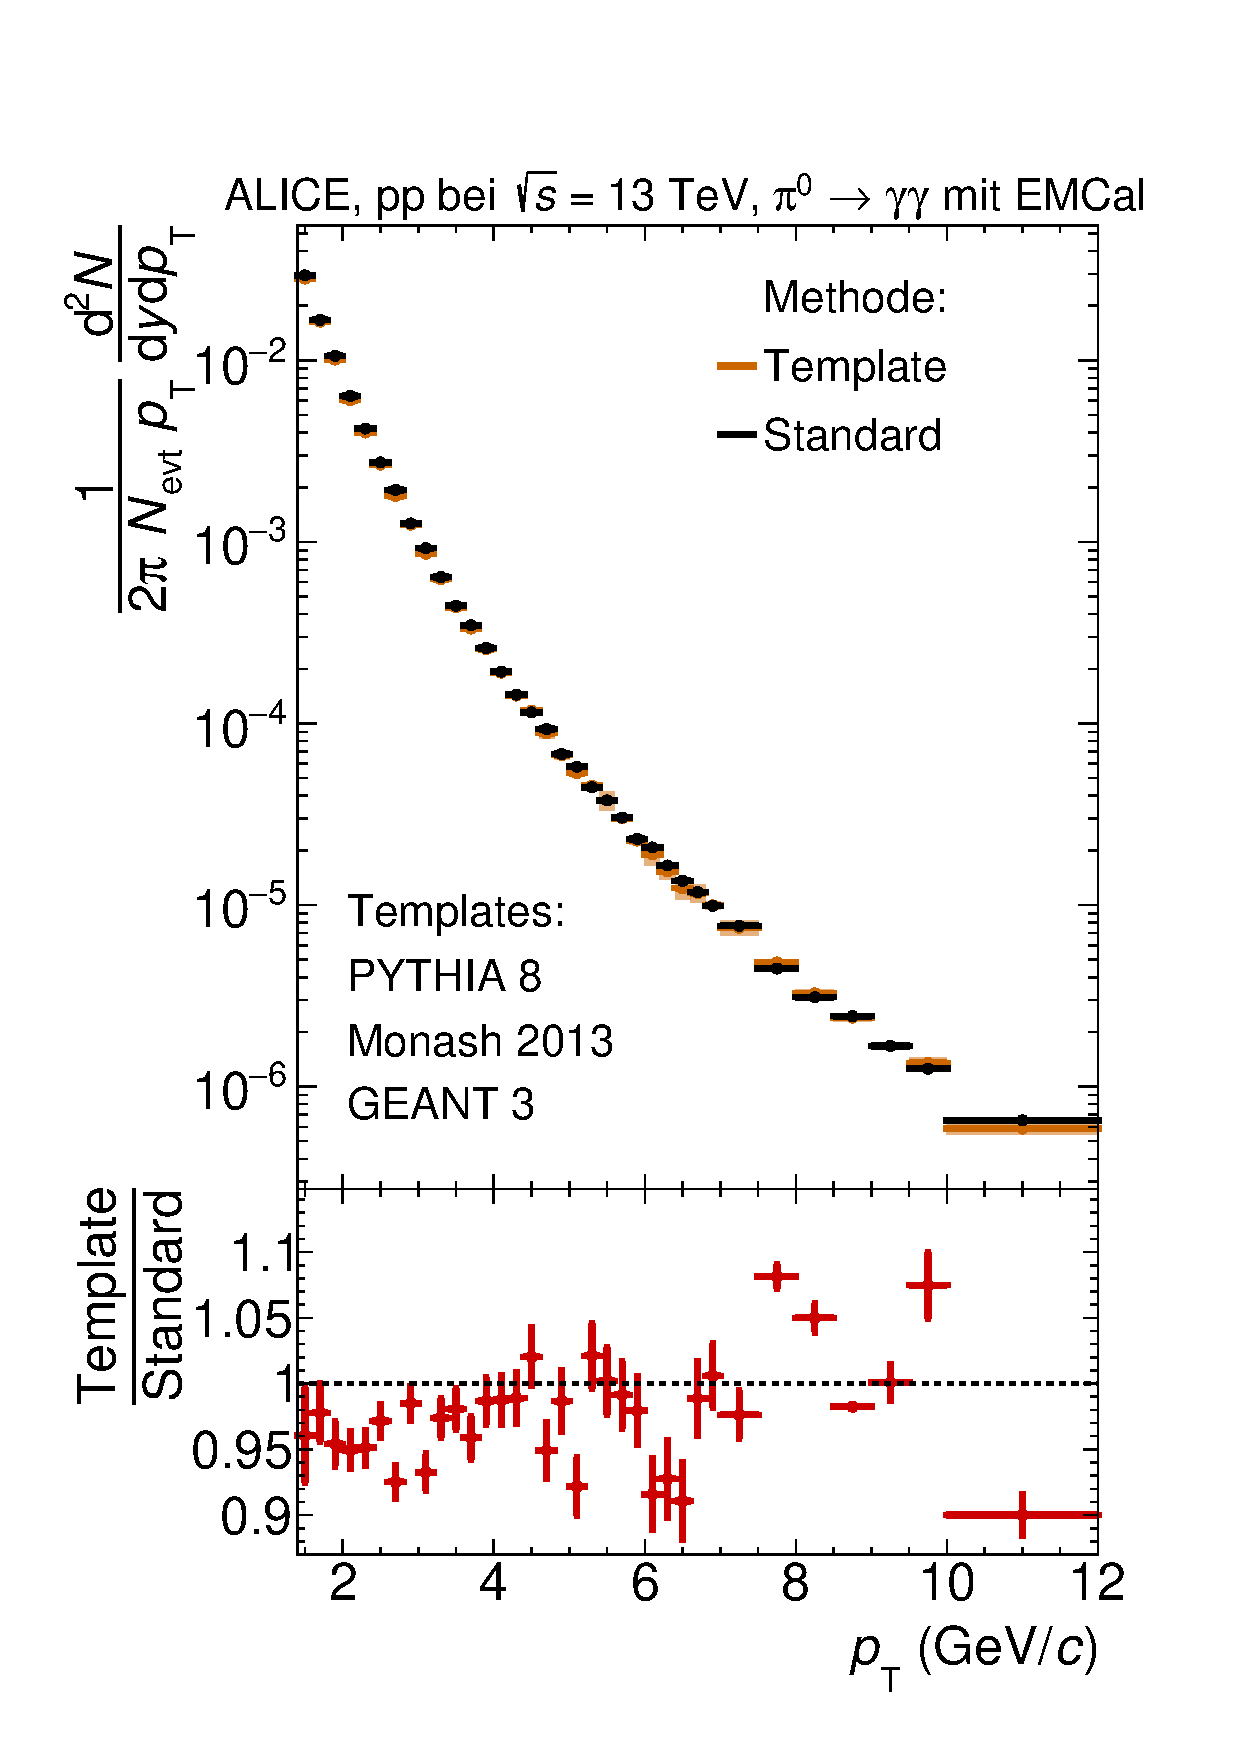
\includegraphics[width=.65\linewidth]{KorrigierteYields_Data_2016.pdf}
\caption{Korrigierte $p_\text{T}$-Spektren aus der Template Methode sowie aus der Standardmethode.
Außerdem das Verhältnis der beiden Spektren.}
\label{fig:KorrYieldComp}
\end{figure}
Abbildung \ref{fig:KorrYieldComp} zeigt das korrigierte $p_\text{T}$-Spektrum aus der Template Methode zusammen mit dem korrigierte $p_\text{T}$-Spektrum aus der Standardmethode.
Außerdem zeigt die Abbildung das Verhältnis der Spektren.
Das Verhältnis zeigt eine Diskrepanz zwischen den beiden Spektren von durchschnittlich etwa $5\%$ auf.
Im Bereich von $3,8 \leq p_\text{T}/\text{ (GeV}/c) < 5,8$ liegt das Verhältnis innerhalb der statistischen Unsicherheiten sogar auf $1$.
Der größte Unterschied zwischen den Spektren beträgt etwa $10\%$, wo die statistischen Unsicherheiten der beiden Spektren den unterschied nicht abdecken.
Mit Hilfe der systematischen Unsicherheiten neben den statistischen sollte sich eine gute Übereinstimmung der beiden Spektren ergeben.
\begin{figure}[t!]
\centering
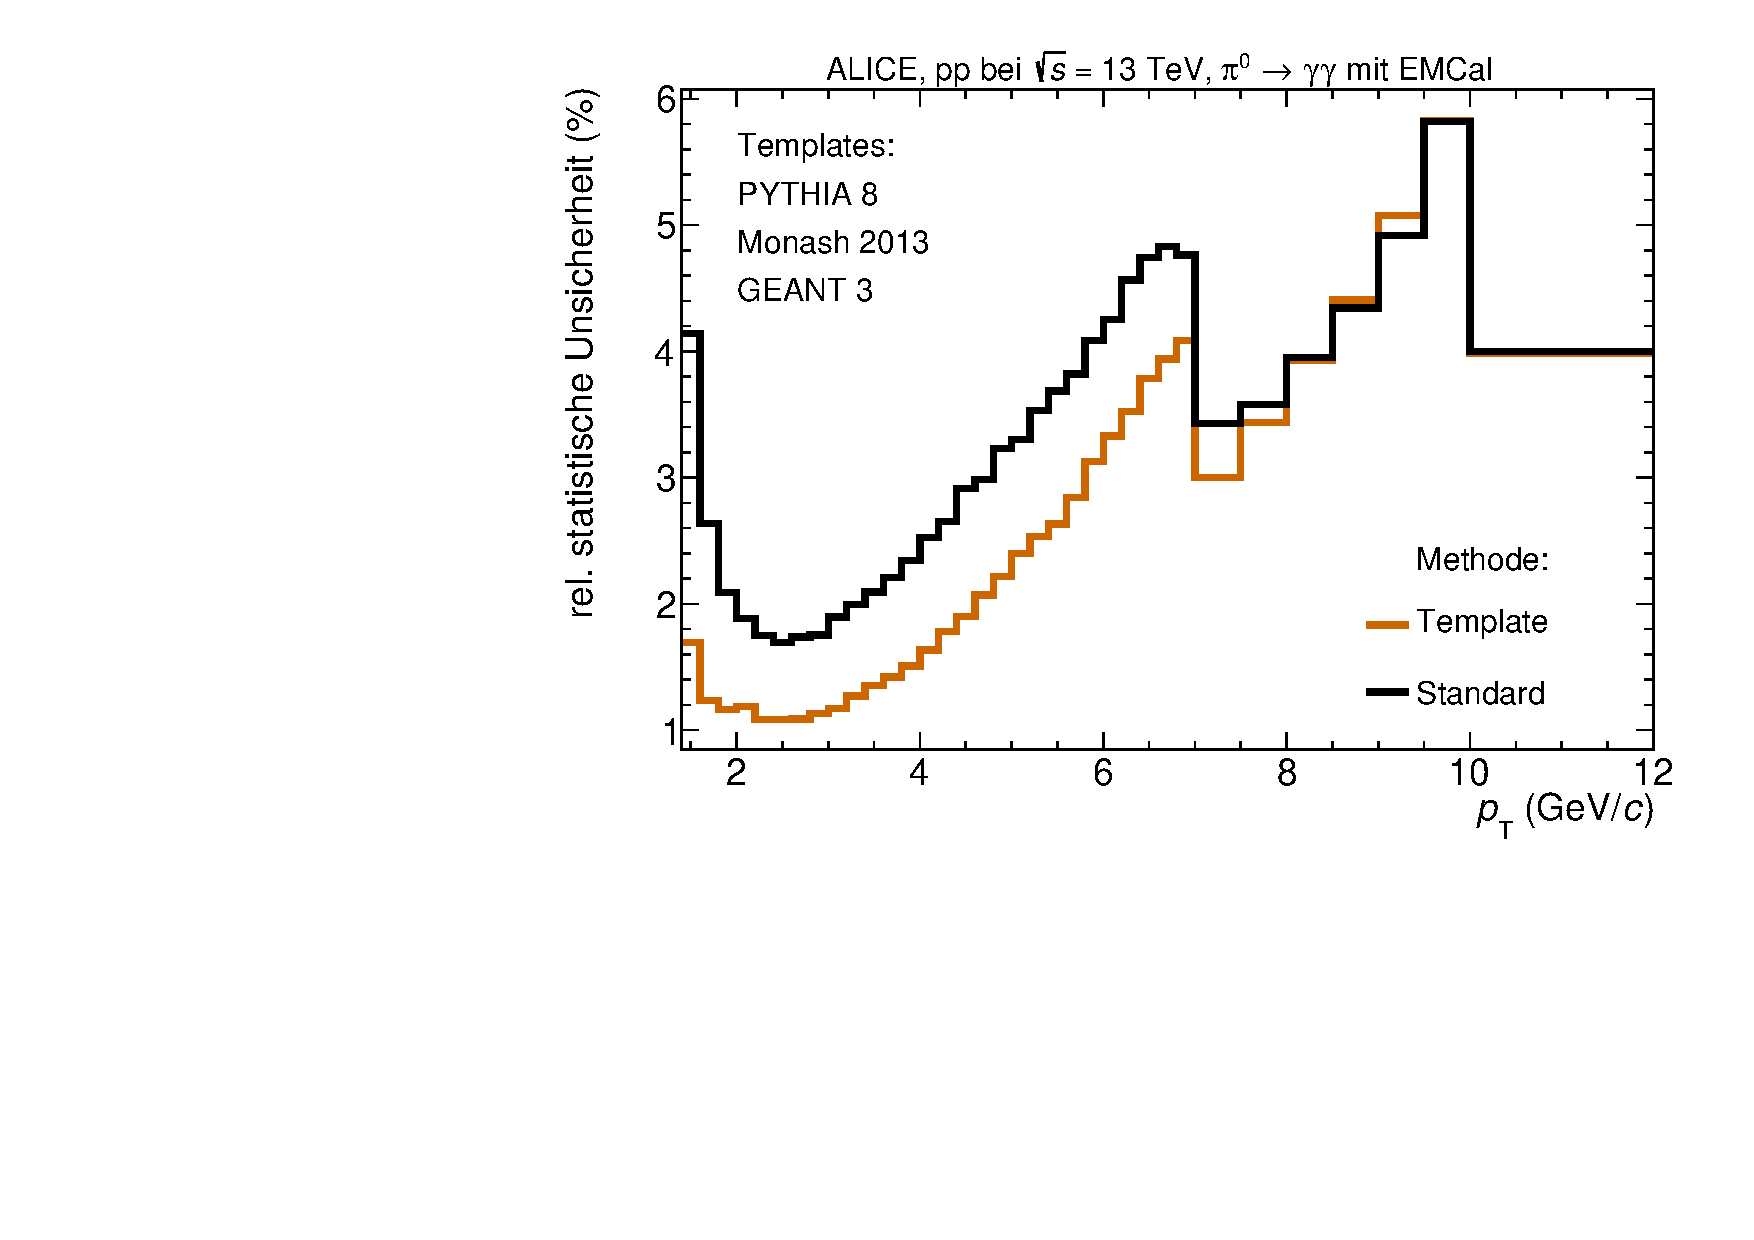
\includegraphics[width=.65\linewidth]{StatistischeUnsicherheitVergleich_Data_2016.pdf}
\caption{Statistische Unsicherheit der korrigierten $p_\text{T}$-Spektren aus der Analysemethode mit Templates, sowie aus der Standardmethode in Abhängigkeit von $p_\text{T}$.}
\label{fig:StatUncer}
\end{figure}
\newline
Abbildung \ref{fig:StatUncer} zeigt die statistischen Unsicherheiten der Spektren der beiden Methoden.
Der Verlauf der statistischen Unsicherheiten weist eine große Ähnlichkeit auf.
Über fast den gesamten $p_\text{T}$-Bereich weist die Template Methode eine geringe statistische Unsicherheit auf, als die Standardmethode.
Die geringere statistische Unsicherheit bei der Template Methode kommt von dem großen Zählbereich, der mit  dieser Methode möglich ist, sowie dem Anteil des Signals, das aus Konversionselektronen und Koversionspositronen besteht.
Zuvor wurde bereits gezeigt, dass die Standardmethode diesen Anteil des Signals unterschätzt.
\newline
Aufgrund der geringeren statistischen Unsicherheit der Template Methode, sowie der guten Über\-ein\-stim\-mung mit der Standardmethode stellt die Tempalte Methode eine mögliche alternative zur Standardmethode dar.
Dabei kann sie entweder als neuer Standard für die Analyse von $\pi^{0}$ in pp-Kollisionen benutzt werden, oder als eine Variation für die Bestimmung der systematischen Unsicherheiten.
\newline
Außerdem zeigt der Vergleich der beiden Methoden, dass die Produktion von $\pi^{0}$ in pp-Kollisionen theoretisch gut verstanden wurde, da die Templates aus einer Monte Carlo Simulation entstanden.